\documentclass{article}
\usepackage{iclr2027_conference,times}
\usepackage{amsmath,amssymb,booktabs,graphicx,microtype,xcolor}
\usepackage{tikz}
\usetikzlibrary{arrows.meta,positioning,calc}
\usepackage{hyperref,url}
\hypersetup{colorlinks=true,citecolor=blue,urlcolor=blue,linkcolor=blue,pdfauthor={Anonymous authors}}


\title{Talking to a Connectome: Language-Model Agents Teach and Interrogate a Whole-Brain Fly Model}
\author{Anonymous authors\\Working research draft}

\begin{document}
\maketitle

\begin{abstract}
Whole-brain connectome models make it possible to run behavioural experiments in silico. We let language-model agents experiment on such a model as an experimenter would: presenting odours, pairing them with sugar or shock, and measuring the fly's approach valence. The model is a leaky integrate-and-fire network of the adult \emph{Drosophila} brain on the FlyWire connectome (138{,}639 neurons) with dopamine-gated plasticity at Kenyon-cell output synapses. Manipulating the model shows that an odour recruits its own dopamine through Kenyon-cell-to-dopamine-neuron synapses, so that presenting it alone changes its memory, that learning changes this dopamine, and that a memory cannot be undone to within tolerance. In open-loop teaching, one pairing per target meets 0.80 of targets (doing nothing meets 0.71), a zero-shot frontier model writes nearly the same protocols, and teachers optimised on a fast surrogate of the fly exploit the surrogate's errors (0.99 predicted, 0.75 measured). In closed-loop diagnosis of a hidden training history from twelve measurements, the main difficulty is generalisation between odours that share Kenyon cells. Claude Sonnet 5 scores 0.832 against 0.793 for a thresholding rule because it respects the stated prior that at most two odours were trained; the rule with that prior scores 0.846. Given a one-page summary of the model's noise and generalisation between odours, and told how answers are scored, Claude reaches 0.894, level with a Bayes player that knows the same (0.912), and gets all seven labels right in 73\% of flies instead of 35\%. Qwen3-32B cannot use the summary, although thirty steps of multi-turn GRPO raise it from 0.765 to 0.830, Claude's zero-shot level. Language-model representations of odour names predict the fly's odour code no better than molecular structure, at 4B or 32B parameters.
\end{abstract}

\section{Introduction}
Connectome-constrained models now cover the whole adult fly brain. A leaky integrate-and-fire (LIF) network wired by the FlyWire connectome \citep{dorkenwald2024,schlegel2024} reproduces feeding and grooming circuits \citep{shiu2024}, and connectome-constrained networks predict activity in the visual system \citep{lappalainen2024} and control a simulated body \citep{jin2026}. These models let behavioural experiments run in silico, but a person still decides which experiment to run and what its outcome means.

Language models are increasingly used as scientific agents, from automated research pipelines \citep{lu2024aiscientist} to text environments for discovery \citep{wang2022scienceworld,jansen2024discoveryworld} and prediction of neuroscience results \citep{luo2025brainbench}. A whole-brain model is an unusual environment for such agents. Its inputs and outputs are those of a wet-lab experiment, but its ground truth is fully specified: the simulator can score every conclusion exactly, which also makes it a source of verifiable rewards for reinforcement learning \citep{shao2024,deepseekr1}.

We build this environment around olfactory associative learning. The agent may present one of seven odours, pair it with sugar or shock (stimulation of reward or punishment dopamine neurons), or measure the fly's approach valence, a summary of mushroom-body output neuron (MBON) activity. The fly learns only through a dopamine-gated rule at Kenyon-cell (KC) to MBON synapses. On this substrate we pose three tasks: teach a target preference profile with an open-loop protocol, diagnose a hidden training history from twelve measurements, and erase a hidden memory.

Our contributions are:
\begin{itemize}
\item A closed-loop experimental environment on a whole-brain spiking model, with tasks whose answers the simulator checks exactly (Section~\ref{sec:env}).
\item Three properties of the substrate, found by manipulating the model, that determine what agents can achieve: odours recruit their own dopamine through KC$\rightarrow$DAN synapses, learning changes that dopamine, and memories cannot be undone to within tolerance (Section~\ref{sec:substrate}).
\item Evidence that open-loop teaching has a simple optimum, which a zero-shot frontier model reproduces, while teachers optimised on a fast surrogate of the fly, by search or by GRPO, exploit the surrogate's errors (Section~\ref{sec:teach}).
\item Closed-loop diagnosis, where the main difficulty is generalisation between odours. A frontier model's lead over a thresholding rule comes from respecting the task's prior; given a summary of the circuit's generalisation and the scoring rule it matches a Bayes player with the same knowledge, which an open 32B model cannot do; and multi-turn GRPO brings the open model to the frontier model's zero-shot level within 30 steps (Section~\ref{sec:diagnose}). A language interface to the fly's odour code aligns with it only through chemistry (Section~\ref{sec:language}).
\end{itemize}

\begin{figure}[t]
\centering
\resizebox{\linewidth}{!}{%
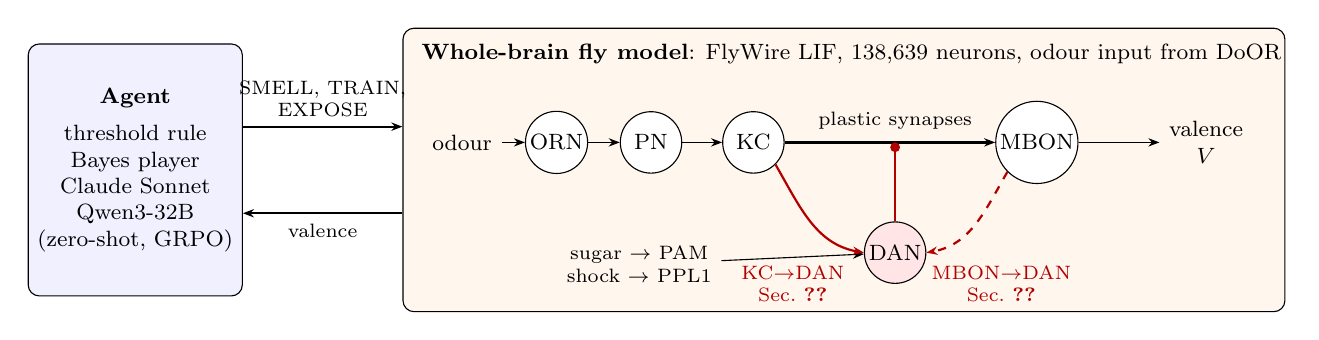
\begin{tikzpicture}[font=\footnotesize, >={Stealth[length=4pt]}, cell/.style={draw, circle, inner sep=1pt, minimum size=0.78cm, fill=white}]
% agent
\node[draw, rounded corners, fill=blue!6, minimum width=2.4cm, minimum height=3.2cm, align=center] (agent) at (0,0)
  {\textbf{Agent}\\[4pt]threshold rule\\Bayes player\\Claude Sonnet\\Qwen3-32B\\(zero-shot, GRPO)};
% fly box
\node[draw, rounded corners, fill=orange!7, minimum width=11.2cm, minimum height=3.6cm] (fly) at (9.0,0) {};
\node[anchor=north west, align=left] at ($(fly.north west)+(0.12,-0.08)$) {\textbf{Whole-brain fly model}: FlyWire LIF, 138{,}639 neurons, odour input from DoOR};
% chain
\node (odour) at (4.15,0.35) {odour};
\node[cell] (orn) at (5.35,0.35) {ORN};
\node[cell] (pn) at (6.55,0.35) {PN};
\node[cell] (kc) at (7.85,0.35) {KC};
\node[cell] (mbon) at (11.45,0.35) {MBON};
\node[align=center] (val) at (13.6,0.35) {valence\\$V$};
\draw[->] (odour) -- (orn); \draw[->] (orn) -- (pn); \draw[->] (pn) -- (kc);
\draw[->, line width=1pt] (kc) -- (mbon);
\node[font=\scriptsize] at (9.65,0.62) {plastic synapses};
\draw[->] (mbon) -- (val);
% dopamine
\node[cell, fill=red!10] (dan) at (9.65,-1.05) {DAN};
\draw[-{Circle[length=3.5pt]}, red!70!black, line width=0.7pt] (dan) -- (9.65,0.35);
\node[align=center, font=\scriptsize] (rf) at (6.4,-1.2) {sugar $\rightarrow$ PAM\\shock $\rightarrow$ PPL1};
\draw[->] (rf) -- (dan);
\draw[->, red!70!black, line width=0.8pt] (kc.south east) to[out=-60, in=170] (dan.west);
\draw[->, red!70!black, dashed, line width=0.8pt] (mbon.south west) to[out=-120, in=10] (dan.east);
\node[font=\scriptsize, red!70!black, align=center] at (8.35,-1.45) {KC$\rightarrow$DAN\\Sec.~\ref{sec:selfda}};
\node[font=\scriptsize, red!70!black, align=center] at (11.0,-1.45) {MBON$\rightarrow$DAN\\Sec.~\ref{sec:dafeedback}};
% agent <-> fly
\draw[->, thick] ($(agent.east)+(0,0.55)$) -- node[above, font=\scriptsize, align=center]{SMELL, TRAIN,\\EXPOSE} ($(fly.west)+(0,0.55)$);
\draw[<-, thick] ($(agent.east)+(0,-0.55)$) -- node[below, font=\scriptsize]{valence} ($(fly.west)+(0,-0.55)$);
\end{tikzpicture}}
\caption{The environment. An agent acts on a whole-brain fly model through odours and reinforcement and observes the approach valence $V$ computed from mushroom-body output neurons (MBON). Dopamine neurons (DAN) gate depression of KC$\rightarrow$MBON synapses. Two pathways into the DANs (red), from Kenyon cells and from MBONs, determine what can be taught and inferred.}
\label{fig:overview}
\end{figure}

\section{Related work}
\textbf{Connectome models.} Whole-brain LIF models on FlyWire reproduce sensorimotor pathways \citep{shiu2024}; connectome-constrained networks predict visual responses \citep{lappalainen2024} and drive locomotion \citep{jin2026}. Interactive repositories couple fly-connectome simulations to games \citep{flyescape} or train connectome-shaped networks on language tasks \citep{flyaslm2026}. We add learning at mushroom-body synapses and study agents that experiment on the model.

\textbf{Mushroom-body learning.} Dopamine neurons innervate MBON compartments and depress KC$\rightarrow$MBON synapses when KC activity and dopamine coincide \citep{aso2014,hige2015}. KCs also synapse onto DANs \citep{li2020}, forming a positive feedback loop required for learning \citep{cervantes2017}, and odour-evoked dopamine underlies familiarity in one compartment \citep{hattori2017}. Models of the mushroom body study reward prediction errors through MBON$\rightarrow$DAN feedback \citep{bennett2021} and similarity-preserving KC codes \citep{dasgupta2017}.

\textbf{Language agents and verifiable rewards.} LLM agents run experiments in text environments \citep{wang2022scienceworld,jansen2024discoveryworld} and carry out research end to end \citep{lu2024aiscientist}. Group-relative policy optimisation (GRPO) trains language models from verifiable rewards without a critic \citep{shao2024,deepseekr1}. Optimising a learned proxy of the reward exploits the proxy's errors \citep{gao2023}; we observe the same with a surrogate of a brain model. Choosing measurements to identify a hidden cause is the problem of Bayesian experimental design \citep{chaloner1995}. LLM agents struggle with experimental design and model discovery \citep{gandhi2025boxinggym}, and they fall short of Bayesian inference when reverse-engineering black-box systems from observations, less so when they can choose their own queries \citep{geng2025blackbox}; our Bayes player gives the same kind of reference for a brain model.

\section{Environment}\label{sec:env}
\textbf{Whole-brain model.} We use the LIF model of \citet{shiu2024} on FlyWire v783 (138{,}639 neurons, 15{,}091{,}983 connections, Brian~2 \citep{stimberg2019}) with four documented corrections: antennal-lobe local neurons are made inhibitory, dopamine neurons have no fast synaptic effect, PN$\rightarrow$KC weights are doubled so that about 7\% of KCs respond to an odour, and KC$\rightarrow$MBON weights are tripled so that both approach and avoidance MBONs respond. The corrections were checked not to change the sugar, grooming and escape pathways validated by \citet{shiu2024} (Appendix~\ref{app:model}). An odour drives each glomerulus's receptor neurons with Poisson input proportional to its DoOR response \citep{munch2016}, 150~Hz at the maximum response. A trial lasts 250~ms. Sugar and shock are 60~Hz stimulation of all PAM or all PPL1 dopamine neurons during the odour, as in classical conditioning \citep{tully1985}.

\textbf{Plasticity and readout.} After every trial, each KC$\rightarrow$MBON synapse $(i,j)$ is depressed by coincident KC and compartment dopamine activity:
\begin{equation}
m_{ij} \leftarrow \max\!\big(m_{\min},\; m_{ij}\,(1-\eta\, a_i\, d_j)\big),\label{eq:rule}
\end{equation}
where $a_i=\min(1, r_i/15\,\text{Hz})$ is the KC rate, $d_j$ is the connectivity-weighted rate of the DANs that synapse on MBON~$j$ (normalised by 20~Hz, zero below 0.3), $\eta=0.6$ and $m_{\min}=0.05$. The rule applies to every trial, including an odour presented alone. The readout is the approach valence $V=(A-B)/(A+B+1)$, where $A$ and $B$ are the summed rates of approach and avoidance MBONs, assigned by transmitter following \citet{aso2014}. Every run is deterministic given its seeds.

\textbf{Odours and tasks.} Seven odours were chosen by a rule fixed before any agent was run: the strongest responder with stable valence from each chemical class (ethyl acetate, 1-hexanol, 2-heptanone, hexanal, acetic acid, linalool), plus methyl acetate, whose KC code overlaps most with that of ethyl acetate (0.81). \emph{Teach}: given a target for every odour (approach more, avoid more, or change $V$ by less than 0.15), write a protocol of at most six trials without feedback. There are 74 test profiles with 1--3 targets, scored by the fraction of odours meeting their target. \emph{Diagnose}: a fly arrives with a hidden history (0, 1 or 2 odours with probability 0.1, 0.45 and 0.45, each paired with sugar or shock 1--3 times in random order). The agent may measure the valence of any odour up to 12 times, each time on a fresh seed and without learning, and then labels each odour $+$, $-$ or $0$. The score averages the fraction of trained odours labelled correctly and the fraction of untrained odours labelled $0$, because most odours are untrained and ``answer all $0$'' would otherwise look strong. \emph{Erase}: on the same flies, use 12 actions (measure, pair, expose) to return every odour's valence to within 0.15 of an untrained fly. All agents receive the same instructions and the same 60 test flies (seeds 0--59); Appendix~\ref{app:tasks} gives the prompts.

\textbf{Agents.} A \emph{threshold rule} measures every odour, re-measures the most ambiguous ones, and labels shifts beyond $\pm0.10$ from the untrained fly. An approximate \emph{Bayes player} enumerates all 799 histories the prior allows, estimates each history's valence distribution for every odour from simulation, measures the odour with the largest posterior predictive variance, and answers either with each odour's most probable label or with the labelling that maximises the expected score. \emph{Claude Sonnet 5} (claude-sonnet-5) is called zero-shot through its command-line interface, one line per turn. \emph{Qwen3-32B} \citep{qwen3} is decoded greedily without thinking, zero-shot and after multi-turn GRPO with LoRA \citep{hu2022} on flies from a disjoint seed range (Appendix~\ref{app:grpo}). For teaching we also fit a fast surrogate of the fly and optimise protocols against it (Section~\ref{sec:teach}).

\section{What the substrate allows}\label{sec:substrate}
\subsection{Odours recruit their own dopamine}\label{sec:selfda}
Presented alone, ethyl acetate activates 13--17 DANs per trial, among them PPL1-$\alpha$3 at 80~Hz and PAM neurons of the $\beta$2 and $\gamma$4 compartments (compartments assigned by DAN$\rightarrow$MBON connectivity). In the connectome, 84\% of the synaptic input weight onto DANs comes from KCs. Under Eq.~\ref{eq:rule} this dopamine depresses synapses without any reinforcement: when odour and reinforcement are presented in separate trials (three of each), ethyl acetate's valence falls from 0.19 to $-0.04$ (Figure~\ref{fig:substrate}a). Cutting all 81{,}056 KC$\rightarrow$DAN connections removes this shift (0.187; each of three seeds within 0.015 of its untrained value), leaves shock learning unchanged ($-0.43$), and strengthens sugar learning from 0.67 to 0.80, because the odour's own PPL1-$\alpha$3 dopamine works against the reward. A KC$\rightarrow$DAN positive feedback loop exists in flies \citep{cervantes2017,li2020}, and odour-evoked dopamine drives familiarity in the $\alpha'$3 compartment \citep{hattori2017}. The model recruits $\alpha$3, $\beta$2 and $\gamma$4 instead, a discrepancy that imaging could test.

\subsection{Learning changes that dopamine}\label{sec:dafeedback}
After three shock pairings, ethyl acetate presented alone activates 10 DANs instead of 17, and after three sugar pairings 25 (Figure~\ref{fig:substrate}b). Methyl acetate changes the same way (16 to 9 and 26); acetic acid loses DANs after either kind of training (19 to 10 and 15; Table~\ref{tab:dan}). Learning changes only KC$\rightarrow$MBON synapses, so these changes must reach the DANs from MBON output, directly or through other neurons: the teaching signal of the next trial depends on what the fly has learned. A fast surrogate that keeps the dopamine of each trial fixed and treats MBON rates as linear in their KC drive fits 40 held-out random protocols well ($r=0.88$, $R^2=0.77$, sign agreement 98\% for changes above 0.15), yet it overrates exactly the trials that optimisers select (Section~\ref{sec:teach}).

\subsection{Memories cannot be undone}\label{sec:erase}
For 20 flies with a single trained odour, knowing the history, we applied $m$ pairings of the opposite sign or $m$ odour-alone exposures (Figure~\ref{fig:substrate}c). One opposite pairing reduces the median deviation from the untrained fly from 0.38 to 0.31; two or more overshoot (0.55--0.65). Exposures leave it at 0.37--0.38. Choosing the best of these 13 strategies for each fly after the fact returns 25\% of trained odours to within 0.15. Eq.~\ref{eq:rule} can only depress synapses, so a memory can be masked by an opposing one but not undone. Erasure is therefore near its floor for every agent: leaving the fly alone scores 0.453, the threshold rule 0.423, a player that knows the history 0.458 and zero-shot Qwen3-32B 0.415 (40 flies). We report it and do not train on it.

\begin{figure}[t]
\centering
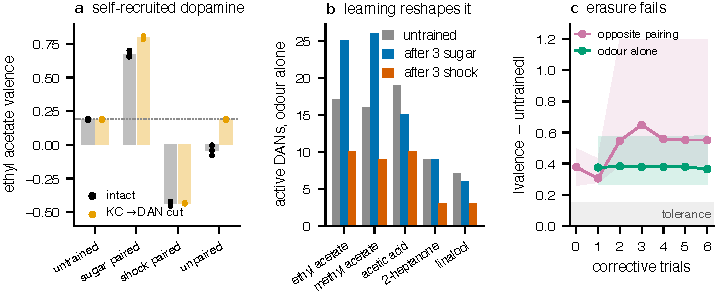
\includegraphics[width=\linewidth]{figures/fig2_substrate.pdf}
\caption{Properties of the substrate. \textbf{a}, Ethyl acetate valence after three sugar pairings, three shock pairings, or odour and reinforcement presented in separate trials (dots: three seeds). Cutting KC$\rightarrow$DAN connections removes the unpaired shift. \textbf{b}, DANs active when the odour is presented alone, before and after three pairings. \textbf{c}, Deviation of a trained odour from the untrained fly after $m$ corrective trials (median and interquartile range, 20 flies); the grey band is the task tolerance.}
\label{fig:substrate}
\end{figure}

\section{Open-loop teaching}\label{sec:teach}
Figure~\ref{fig:teach} compares teachers on the 74 target profiles, all scored on the whole-brain model with fixed training and probe seeds (full results in Table~\ref{tab:teach}). Doing nothing meets every ``unchanged'' target and scores 0.707. Pairing each target once, with sugar for ``approach more'' and shock for ``avoid more'', scores 0.799 and solves 18.9\% of profiles completely with 2.1 trials on average. Claude Sonnet, given only the task text, writes nearly the same protocols (2.3 trials) and scores 0.793. Repeating the pairings to fill the six-trial budget moves the targets more (0.90 of targets against 0.86) but disturbs the untouched odours (0.62 kept against 0.78) and scores 0.701: generalisation through shared Kenyon cells makes every extra trial a side effect (Figure~\ref{fig:teach}b). Searching on the fly itself over 1--3 pairings per target, with separate selection seeds, scores 0.786. The one-pairing rule fails most often on ethyl acetate: a single sugar pairing makes the fly approach it more in 1 of 10 profiles (mean change $+0.075$), in line with Section~\ref{sec:selfda}, where the odour's own PPL1-$\alpha$3 dopamine weakens sugar learning.

Teachers optimised on the surrogate fail on the fly. Beam search over the surrogate finds protocols it predicts to score 0.988; they score 0.749. Of their trials, 35\% are odour-alone exposures, which the surrogate treats as a cheap way to lower valence. On the fly such exposures lowered a target by 0.11 on average (target met in 30\% of cases), against 0.47 for a shock pairing (84\%). Running the surrogate's 16 best proposals per profile on the fly with separate seeds and keeping the best raises the score to 0.774. GRPO on the surrogate teaches Qwen3-0.6B to reach 0.82 on validation profiles as judged by the surrogate; on the fly its test protocols score 0.770 (0.857 predicted). All 74 of them begin with a sugar pairing of ethyl acetate and 61\% of their trials are exposures, so the policy moves only 46\% of its targets and scores mainly by leaving untouched odours alone. GRPO with rewards from the fly itself brought Qwen3-0.6B and Qwen3-4B-Base only to the level of doing nothing on the validation profiles (Appendix~\ref{app:teachgrpo}). Open-loop teaching has a simple optimum, and a surrogate that ignores the dopamine feedback of Section~\ref{sec:dafeedback} steers optimisers away from it.

\begin{figure}[t]
\centering
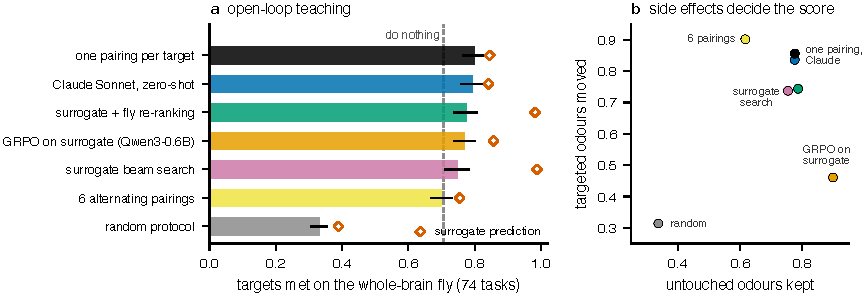
\includegraphics[width=\linewidth]{figures/fig3_teaching.pdf}
\caption{Open-loop teaching. \textbf{a}, Fraction of targets met on the whole-brain model (bars, 95\% bootstrap intervals over the 74 profiles) and as predicted by the surrogate (diamonds); the dashed line is the score of doing nothing. \textbf{b}, Targeted odours moved in the required direction versus untouched odours kept within tolerance; colours as in \textbf{a}.}
\label{fig:teach}
\end{figure}

\section{Closed-loop diagnosis}\label{sec:diagnose}
Diagnosis requires the agent to act on what the fly reports. Figure~\ref{fig:diagnose} and Table~\ref{tab:diagnose} compare players on the same 60 flies. Answering $0$ everywhere scores 0.533 and random play 0.309. The threshold rule scores 0.793 (all seven labels right for 23\% of flies): it finds 95\% of trained odours but labels 36\% of untrained odours as trained. Most of these false alarms are real shifts, not noise. By the Bayes player's table, 111 of the 333 untrained odour--fly pairs in the test set have an expected valence shift above 0.10, caused by training another odour that shares Kenyon cells with it, and the rule labels 102 of these 111 as trained but only 14 of the other 222 (Table~\ref{tab:errors}). Measurement noise matters for two odours: in the untrained fly the valence of linalool varies with SD 0.12 between measurements and that of hexanal with 0.06, the others with at most 0.024. Zero-shot Qwen3-32B scores 0.765 and makes both kinds of error: it labels as trained 66 of the 111 generalised odours and 52 of the 222 unshifted ones.

Claude Sonnet 5 scores 0.832 [0.785, 0.880] with 8.4 measurements on average. Against the rule on the same flies it wins 31 times and loses 16 times (paired difference $+0.039$, 95\% bootstrap interval $[-0.002, 0.079]$, permutation $p=0.07$). Its advantage comes from a fact stated in the task: up to two odours were trained. Claude never labels more than two odours as trained, whereas the rule does so in 43 of 60 flies and zero-shot Qwen3-32B in 42. Adding this constraint to the rule after the fact, on the rule's own measurements, gives 0.846 [0.795, 0.894], ties Claude's score on 48 of 60 flies, and cuts the rule's errors on generalised odours from 102 to 34. GRPO moves Qwen3-32B the same way. After 30 steps (240 training flies) it scores 0.830 [0.784, 0.873], $+0.065$ over zero-shot on the same flies (95\% interval $[0.013, 0.121]$, permutation $p=0.02$), level with Claude ($-0.002$), and gets all seven labels right in 32\% of flies instead of 7\%. It labels more than two odours in 14 flies instead of 42, and its errors fall from 52 to 10 on unshifted odours and from 66 to 42 on generalised ones, at the cost of missing more trained odours (21 of 87 instead of 8).

The measurements contain more than the zero-shot agents extract. The approximate Bayes player, which knows the response statistics of every possible history, scores 0.912 [0.876, 0.944] with 12 measurements when it answers to maximise the expected balanced score, 0.079 above Claude (paired interval $[0.023, 0.138]$). Answering instead with each odour's most probable label, it scores 0.845 and gets all seven labels right in 63\% of flies. It separates direct from generalised shifts by their size and pattern: it misses 9 of 87 trained odours and labels 29 of the 111 generalised odours as trained. One confusion remains for all these players, the Bayes player included: when only one of the two esters was trained, the other is labelled trained in 10 to 14 of the 15 such flies. With KC codes that overlap by 0.81, the two esters are nearly indistinguishable through the valence.

To separate knowledge from inference, we gave the language agents what the Bayes player knows, as a one-page brief computed from its table: the measurement noise of each odour and the average change of every odour after one or three pairings of each odour with sugar or with shock (Appendix~\ref{app:diagnose}). With the brief, Claude answers like the Bayes player. It scores 0.845 [0.788, 0.898], the same as the Bayes player with most probable labels (paired difference $0.000$, $[-0.055, 0.057]$), and gets all seven labels right in 60\% of flies instead of 35\% (18 flies gained, 3 lost, McNemar $p=0.002$). Its errors match that player's: 18 of the 111 generalised odours labelled trained (Bayes player 19) and 24 of 87 trained odours missed (24). Its labelling is identical in 38 of 60 flies, against 15 without the brief, although Claude chose its own 8.8 measurements. The ester confusion falls to 7 of 15 flies, a difference from the Bayes player's 10 that 15 flies cannot resolve. The task text does not say how answers are scored, and Claude's answers match those of the Bayes player that maximises the number of correct labels. Told in addition how answers are scored, Claude with the brief scores 0.894 [0.840, 0.942], level with the Bayes player tuned to the score (paired difference $-0.018$, $[-0.074, 0.037]$). It gets all seven labels right in 73\% of flies (Bayes player 57\%), labels 11 of the 111 generalised odours as trained, misses 17 of 87 trained odours and confuses the esters in 5 of 15 flies, with 9.0 measurements instead of 12. The scoring rule alone does not help: told how answers are scored but given no brief, Claude scores 0.821 [0.767, 0.871] with all seven labels right in 33\% of flies. Qwen3-32B does not use the brief: zero-shot it scores 0.751 with the brief and 0.765 without, and the policy after 30 GRPO steps 0.788 against 0.830.

\begin{figure}[t]
\centering
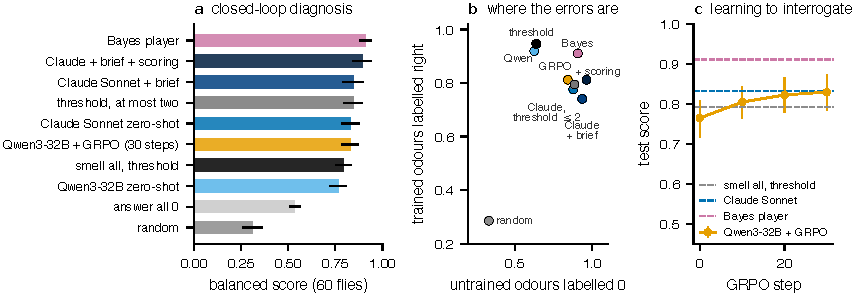
\includegraphics[width=\linewidth]{figures/fig4_diagnose.pdf}
\caption{Closed-loop diagnosis on 60 flies. \textbf{a}, Balanced score with 95\% bootstrap intervals over flies. \textbf{b}, Trained odours labelled correctly versus untrained odours labelled $0$; colours as in \textbf{a}. \textbf{c}, Test score of Qwen3-32B during GRPO; dashed lines mark other players.}
\label{fig:diagnose}
\end{figure}

\begin{table}[t]
\centering
\caption{Diagnosis on 60 flies (seeds 0--59). Score averages trained odours labelled right and untrained odours labelled $0$; exact means all seven labels right. Intervals are 95\% bootstrap over flies. $^\ast$Added after the first results: decision rules applied to the recorded measurements of the threshold rule and of the Bayes player, and runs with the brief or the scoring rule added to the prompt (Appendix~\ref{app:diagnose}). The Bayes player knows the response statistics of all 799 histories.}
\label{tab:diagnose}
\footnotesize
\begin{tabular}{lccccc}
\toprule
Player & Score [95\% CI] & Exact & Trained & Untrained & Measurements \\
\midrule
Random & 0.309 [0.259, 0.365] & 0.00 & 0.29 & 0.33 & 2.9 \\
Answer all $0$ & 0.533 [0.508, 0.567] & 0.07 & 0.00 & 1.00 & 0 \\
Qwen3-32B, zero-shot & 0.765 [0.717, 0.808] & 0.07 & 0.92 & 0.63 & 11.1 \\
Threshold rule & 0.793 [0.753, 0.834] & 0.23 & 0.95 & 0.64 & 12 \\
Qwen3-32B, 30 GRPO steps & 0.830 [0.784, 0.873] & 0.32 & 0.81 & 0.84 & 10.0 \\
Claude Sonnet 5, zero-shot & 0.832 [0.785, 0.880] & 0.35 & 0.78 & 0.88 & 8.4 \\
Threshold rule, $\le 2$ odours$^\ast$ & 0.846 [0.795, 0.894] & 0.43 & 0.79 & 0.89 & 12 \\
\midrule
Claude, scoring rule$^\ast$ & 0.821 [0.767, 0.871] & 0.33 & 0.78 & 0.86 & 8.4 \\
Claude, brief$^\ast$ & 0.845 [0.788, 0.898] & 0.60 & 0.74 & 0.94 & 8.8 \\
Claude, brief + scoring$^\ast$ & 0.894 [0.840, 0.942] & 0.73 & 0.81 & 0.96 & 9.0 \\
Qwen3-32B, brief$^\ast$ & 0.751 [0.677, 0.817] & 0.13 & 0.84 & 0.67 & 11.1 \\
Qwen3-32B, GRPO, brief$^\ast$ & 0.788 [0.736, 0.838] & 0.25 & 0.80 & 0.77 & 10.2 \\
\midrule
Bayes, marginal labels & 0.845 [0.786, 0.900] & 0.63 & 0.73 & 0.94 & 12 \\
Bayes, balanced decision$^\ast$ & 0.912 [0.876, 0.944] & 0.57 & 0.91 & 0.91 & 12 \\
\bottomrule
\end{tabular}
\end{table}

\section{A language interface to the odour code}\label{sec:language}
Can a language model's representation of an odour name stand in for the odour? We mapped Qwen3 hidden states for each DoOR odorant name to glomerular input with ridge regression trained on 688 odorants, ran the predicted input through the brain model, and asked whether the evoked activity is closest to that of the named odorant among 111 held-out odorants with complete receptor data (Appendix~\ref{app:language}). From the name alone, the true odorant has median rank 12 at the input and 16--24 from receptor neurons to the lateral horn and MBONs (chance 56). Morgan fingerprints of the molecule do as well, and character n-grams of the name nearly as well. The reverse map, from the fly's code into the language model's space, works best from the lateral horn (median rank 19). Representational similarity with the fly's code is weak from the input to the lateral horn (Spearman $\rho=0.12$--$0.17$), lower than for molecular structure (0.15--0.22), and near zero at MBONs (0.05). A 32B model does not change this (glomerular prediction $r=0.458$ against 0.461 for 4B at the middle layer). For everyday words the embedding route fails a pre-registered test (the key compound of 25 smells has median rank 45 of 111). In an exploratory follow-up, asking Qwen3-32B to name the compound and letting the fly smell it gives median rank 1: the interface works through the model's knowledge of chemistry, not through representations shared with the fly.

\section{Discussion and limitations}
A connectome model with a single plasticity rule already poses experimental problems that separate agents, and the difficulty comes from the circuit: odours share Kenyon cells, odours recruit their own dopamine, and learned output feeds back on the teaching signal. The same properties make a fast surrogate an unreliable target for optimisation, the brain-model counterpart of reward over-optimisation \citep{gao2023}. Protocols optimised on a model of the fly model should be checked on the fly model, and the same holds between models of flies and flies. Where the language agents did well, they applied a simple rule: one pairing per target when teaching, and at most two trained odours when diagnosing. Claude Sonnet found both from the task text, and 30 GRPO steps moved Qwen3-32B most of the way to the second (more than two odours labelled in 14 of 60 flies instead of 42). Neither agent inferred from twelve measurements how training generalises between odours. Given that knowledge as a table, Claude used it as a Bayesian observer would, and with the scoring rule it matched the Bayes player tuned to the score; Qwen3-32B did not use the table. What limited the first model was knowledge of the circuit, and what limited the second was the ability to use it.

The findings concern a model, not an animal. The plasticity rule has no recovery term; the valence summarises MBON groups rather than behaviour; the four weight corrections were tuned to reported KC sparseness and MBON responses; and in a point-neuron model, axo-axonal KC$\rightarrow$DAN synapses drive DAN spikes directly, which sets the size of the effect in Section~\ref{sec:selfda}. We used one panel of seven odours and 60 test flies, so differences of 0.04 between agents are at the edge of what this sample resolves. The prior-constrained rule, the balanced Bayes decision, the brief and the scoring rule were added after we saw the first results. The task text says that repeated measurements differ by a few hundredths, which understates the noise for odours with weak MBON drive; all language agents saw the same text. Claude was called through a command-line interface without control of sampling, and GRPO ran for 30 steps.

\section*{Reproducibility statement}
The code for the brain model, the environment, all agents and all analyses, the task seeds, the recorded episodes and the scripts that produce every figure and table will be released. All simulations are deterministic given seeds; a replay of a reference trial on a second machine with the same library versions reproduced its spike counts exactly (1{,}498 active neurons, 27{,}898 spikes).

\section*{AI use statement}
An LLM coding agent (Claude) wrote most of the code, ran the experiments and analyses, and drafted the text under the direction of the authors, who take responsibility for the content. Claude Sonnet and Qwen3 models are also experimental subjects of the paper, as described in Section~\ref{sec:env}.

\bibliography{references}
\bibliographystyle{iclr2027_conference}

\appendix
\section{Model details}\label{app:model}
\textbf{Neurons and synapses.} The network follows \citet{shiu2024}: current-based LIF neurons with $v_0=v_{\mathrm{reset}}=-52$~mV, threshold $-45$~mV, membrane time constant 20~ms, synaptic-current decay 5~ms, refractory period 2.2~ms and transmission delay 1.8~ms. A synapse's weight is its FlyWire v783 synapse count times 0.275~mV, with the sign of the predicted transmitter of the presynaptic neuron.

\textbf{Corrections.} Four synapse classes deviate from this rule. Each was checked not to change the three pathways validated by \citet{shiu2024}: sugar to the MN9 motor neuron, Johnston's organ to antennal grooming, and looming to the giant fibre.
\begin{itemize}
\item Antennal-lobe local neurons: outputs of LNs with a predicted monoamine transmitter are made inhibitory and outputs of LNs predicted cholinergic are removed. Almost all LNs are GABAergic; with the original rule one glomerulus recruited all 330 uniglomerular PNs.
\item Dopamine neurons have no fast synaptic effect; dopamine acts only through Eq.~\ref{eq:rule}.
\item PN$\rightarrow$KC weights $\times2$, so that about 7\% of KCs respond to an odour (5--10\% is reported in flies); with $\times1$ fewer than 3\% respond.
\item KC$\rightarrow$MBON weights $\times3$, so that both glutamatergic and cholinergic MBONs respond to odours; with $\times1$ only three GABAergic $\gamma$-lobe MBONs fire.
\end{itemize}
These are implementation choices and not a biological validation.

\textbf{Inputs.} An odour drives the receptor neurons of each glomerulus with Poisson input at 150~Hz times its DoOR response \citep{munch2016}; responses below 0.05 and unmeasured glomeruli give no drive. Sugar is 60~Hz Poisson input to all PAM neurons and shock the same input to all PPL1 neurons, delivered together with the odour.

\textbf{Plasticity.} The DANs of MBON~$j$ are those with at least three synapses onto it, weighted by synapse count and normalised to sum to one; $d_j=\min(1,\sum_k w_{jk} r_k/20\,\mathrm{Hz})$ and $d_j=0$ if $d_j<0.3$. Eq.~\ref{eq:rule} multiplies the corrected weight, and a fly's memory is the vector of factors $m_{ij}$, saved and reloaded exactly.

\textbf{Valence.} Cholinergic MBONs and the GABAergic MBON11 count as approach, glutamatergic MBONs as avoidance \citep{aso2014}, and other GABAergic MBONs are left out. $V=(A-B)/(A+B+1)$ with $A$, $B$ the summed firing rates in Hz over a 250~ms trial.

\textbf{KC$\rightarrow$DAN cut.} Setting all 81{,}056 KC$\rightarrow$DAN connection rows to zero reduces the DANs active in an odour-alone trial of ethyl acetate from 13--17 to 5--7 and the synapses changed per trial from 830--2{,}393 to 77--135. Of the DANs this odour recruits, PPL106 (PPL1-$\alpha$3; 465 synapses onto MBON14) fires at 80~Hz, PAM04 (onto MBON02 and MBON24) at 14~Hz and PAM08 (onto MBON05) at 15~Hz. In a point-neuron model, axo-axonal KC$\rightarrow$DAN synapses in the lobes drive DAN spikes directly, so the size of this effect depends on that simplification.

\begin{table}[h]
\centering
\caption{DANs active in an odour-alone trial, in an untrained fly and after three pairings of the same odour with sugar or shock (seed-matched probes).}
\label{tab:dan}
\small
\begin{tabular}{lccc}
\toprule
Odour & Untrained & After 3 sugar & After 3 shock \\
\midrule
ethyl acetate & 17 & 25 & 10 \\
methyl acetate & 16 & 26 & 9 \\
acetic acid & 19 & 15 & 10 \\
2-heptanone & 9 & 9 & 3 \\
1-hexanol & 8 & 5 & 5 \\
hexanal & 5 & 8 & 3 \\
linalool & 7 & 6 & 3 \\
\bottomrule
\end{tabular}
\end{table}

\section{Tasks, prompts and scoring}\label{app:tasks}
\textbf{Panel.} The rule was fixed before any teaching result: odours with stable valence and at least 40 spikes in the MBONs that enter $V$, the strongest responder of each chemical class, plus the odour whose KC code overlaps most with ethyl acetate (methyl acetate, 0.81). A first rule that used only response strength gave five esters and was replaced before any results.

\textbf{Teaching.} The 74 test profiles are all 14 single targets, all 42 ordered pairs (one odour up, one down) and 18 distinct random triples. Another 274 profiles of 1--3 targets are used for training and 30 for validation. Training trial $t$ uses seed $5000+t$; the panel is then probed on seeds 101--103 without learning. A target is met if $V$ moves by at least 0.15 in the required direction, or by less than 0.15 for ``unchanged''. Every teacher receives this prompt, with the profile filled in:
{\scriptsize
\begin{verbatim}
A fruit fly will be trained with classical conditioning and then tested on each odour.
Odours: ethyl acetate, methyl acetate, 1-hexanol, 2-heptanone, hexanal, acetic acid,
linalool.

Goal for the test after training, compared with the same fly before training:
- ethyl acetate: approach MORE than now
- methyl acetate: stay UNCHANGED
...
You may give at most 6 trials. Each trial is one line in exactly one of these forms:
TRAIN <odour> + REWARD    (the odour is paired with sugar)
TRAIN <odour> + PUNISH    (the odour is paired with an electric shock)
EXPOSE <odour>            (the odour alone, nothing else)

Write only the trial lines, nothing else.
\end{verbatim}}

\textbf{Diagnosis and erasure.} A hidden history picks $k\in\{0,1,2\}$ odours with probability 0.1, 0.45 and 0.45, gives each a sign and 1--3 pairings, and applies the pairings in random order with random seeds, all determined by the fly's seed. A measurement probes the odour on a fresh seed without learning and returns ``The fly's approach valence for linalool: +0.17 (11 actions left)''. The diagnosis score is $\frac12(\text{trained odours labelled with the right sign}+\text{untrained odours labelled }0)$, and flies with $k=0$ score their untrained term alone. The erasure score is $\frac12(\text{trained odours restored to within }0.15+\text{untrained odours kept within }0.15)$. The diagnosis prompt, which every language agent receives:
{\scriptsize
\begin{verbatim}
You are working with a fruit fly in an olfactory learning experiment. Its response to an
odour is measured as an approach valence: positive means it tends to approach the odour,
higher means it likes it more. Pairing an odour with sugar raises the valence for that
odour; pairing it with an electric shock lowers it. Repeated measurements of the same
odour differ by a few hundredths.

Before you got this fly it may have been trained: up to two of the odours below were each
paired with sugar or with shock, one to three times. You do not know which, if any.

Valence of a typical untrained fly:
- ethyl acetate: +0.19
- methyl acetate: +0.17
- 1-hexanol: +0.30
- 2-heptanone: +0.27
- hexanal: +0.35
- acetic acid: +0.15
- linalool: +0.38

Your task: find out how this fly was trained. You have 12 measurements. Each turn, write
exactly one line:
SMELL <odour>
When you are ready (or out of measurements), write ANSWER on the first line followed by
one line per odour:
<odour>: +   (paired with sugar)
<odour>: -   (paired with shock)
<odour>: 0   (not trained)
\end{verbatim}}
The erasure prompt replaces the task paragraph with the goal of matching the untrained fly within 0.15 and adds \texttt{TRAIN <odour> + REWARD}, \texttt{TRAIN <odour> + PUNISH}, \texttt{EXPOSE <odour>} and \texttt{FINISH}. A missing label counts as wrong.

\section{Open-loop teaching}\label{app:teachgrpo}
\textbf{Surrogate.} The surrogate copies Eq.~\ref{eq:rule}, records the KC and DAN rates of each odour, reinforcement and seed in the untrained fly, and assumes that (i) these rates do not depend on memory, which ignores MBON$\rightarrow$DAN feedback, and (ii) each MBON's rate changes linearly with its KC drive, with one fitted slope per MBON. On 40 held-out random protocols run on the brain model it predicts the change in $V$ with $r=0.88$ and $R^2=0.77$ (mean absolute error 0.079; SD of the changes 0.30), and it gets the sign right in 98\% of changes larger than 0.15. Assumption (i) is wrong (Table~\ref{tab:dan}).

\textbf{Teachers.} Beam search (width 48) maximises surrogate success over protocols of up to six trials. Re-ranking runs the surrogate's 16 best protocols per profile on the brain model with training seeds 7000+ and probe seed 301 and keeps the best one. Structured search tries 1--3 pairings per target on the brain model, chosen on the same selection seeds. All teachers are scored on the test seeds.

\begin{table}[h]
\centering
\caption{Teachers on the 74 test profiles, scored on the brain model. Success is the pre-registered fraction of odours meeting their target; moved and kept split it into targeted and untouched odours.}
\label{tab:teach}
\small
\begin{tabular}{lcccccc}
\toprule
Teacher & Success & Solved & Moved & Kept & Trials & Surrogate \\
\midrule
Do nothing & 0.707 & 0\% & 0.00 & 1.00 & 0 & 0.707 \\
One pairing per target & 0.799 & 18.9\% & 0.86 & 0.78 & 2.1 & 0.846 \\
Claude Sonnet, zero-shot & 0.793 & 18.9\% & 0.84 & 0.78 & 2.3 & 0.842 \\
Structured search on the fly & 0.786 & 18.9\% & 0.86 & 0.75 & 3.4 & 0.844 \\
Surrogate + fly re-ranking & 0.774 & 13.5\% & 0.74 & 0.79 & 5.7 & 0.983 \\
GRPO on surrogate (Qwen3-0.6B) & 0.770 & 9.5\% & 0.46 & 0.90 & 5.4 & 0.857 \\
Surrogate beam search & 0.749 & 12.2\% & 0.74 & 0.75 & 5.7 & 0.988 \\
Six alternating pairings & 0.701 & 8.1\% & 0.90 & 0.62 & 6.0 & 0.755 \\
Qwen3-4B-Base, zero-shot & 0.349 & 0\% & 0.63 & 0.23 & 5.7 & 0.361 \\
Random protocol & 0.331 & 0\% & 0.31 & 0.34 & 6.0 & 0.389 \\
Qwen3-0.6B, zero-shot & 0.178 & 0\% & 0.51 & 0.04 & 6.0 & 0.203 \\
\bottomrule
\end{tabular}
\end{table}

Leaving the fly untrained meets every ``unchanged'' target, so it scores 0.707 on the test profiles. With one pairing per target, ``approach more'' succeeds for ethyl acetate in 1 of 10 profiles (mean change $+0.075$), for linalool in 4 of 11 ($+0.168$) and for methyl acetate in 9 of 10 ($+0.174$).

\textbf{GRPO.} Qwen3-0.6B and Qwen3-4B-Base with LoRA (rank 32, all attention and MLP projections), 16 profiles $\times$ 8 samples per step, reward $=$ success $+\,0.2\times$ graded success $-\,0.05\times$ invalid lines, one AdamW step per batch (so the PPO ratio is 1), KL coefficient 0.02 to the base model, at most 80 new tokens; lr $2\times10^{-5}$ for Qwen3-0.6B and $10^{-5}$ for Qwen3-4B-Base, which reads a plain-text prompt without the chat template. The brain-model runs were stopped after 59, 12 and 16 steps when we moved to the closed-loop tasks. Table~\ref{tab:teachgrpo} lists validation success on the 30 validation profiles, which mostly have three targets, so doing nothing scores 0.595 on them. With the surrogate as reward, validation success judged by the surrogate rises to 0.82, and the best checkpoint scores 0.770 on the brain model on the test profiles: every one of its 74 protocols begins with a sugar pairing of ethyl acetate, and 61\% of its trials are odour-alone exposures. With rewards from the brain model (probe seed 201, training seeds 6000--9000), Qwen3-0.6B stalls at the do-nothing level and Qwen3-4B-Base reaches 0.56 after 10 steps. Starting the brain-model run from the surrogate-trained adapter (0.667 at step 0) lowers validation success to 0.619 after 10 steps.

\begin{table}[h]
\centering
\caption{GRPO for teaching: success on the 30 validation profiles (doing nothing scores 0.595).}
\label{tab:teachgrpo}
\small
\begin{tabular}{llcccccc}
\toprule
Model & Reward & step 0 & 10 & 20 & 50 & 100 & 150 \\
\midrule
Qwen3-0.6B & surrogate & 0.281 & 0.595 & 0.595 & 0.657 & 0.805 & 0.824 \\
Qwen3-0.6B & brain model & 0.314 & 0.562 & 0.552 & 0.552 & -- & -- \\
Qwen3-0.6B, surrogate start & brain model & 0.667 & 0.619 & -- & -- & -- & -- \\
Qwen3-4B-Base & brain model & 0.438 & 0.562 & -- & -- & -- & -- \\
\bottomrule
\end{tabular}
\end{table}

\section{Multi-turn GRPO for diagnosis}\label{app:grpo}
We fine-tune Qwen3-32B (bf16, gradient checkpointing) with LoRA (rank 16, $\alpha=32$, no dropout) on the q, k, v, o, gate, up and down projections. Each step plays 8 new flies (history seeds drawn uniformly from $[1000, 10^6)$) with 4 sampled episodes per fly (temperature 0.7, top-$p$ 1), 32 episodes in all; thinking is off, a turn may generate up to 96 tokens, an episode has at most 14 turns, and the last turn is forced to \texttt{ANSWER}. The reward is the episode's diagnosis score. The advantage is the score normalised by the mean and standard deviation of the fly's 4 episodes and applies to every generated token; observation tokens are masked, and the trained token sequence is identical to the generated one. We take one AdamW step per batch (lr $3\times10^{-5}$, betas 0.9/0.99, no weight decay, gradient-norm clip 1.0), so the PPO ratio is 1, and add a per-token k3 KL penalty (coefficient 0.02) towards the base model, normalising the loss by the number of generated tokens. Training ran on one NVIDIA RTX PRO 6000 Blackwell (96~GB) with 40 simulator workers on the same machine. Test evaluation is greedy on seeds 0--59. A first run at temperature 1.0 and lr $10^{-5}$ was stopped after 5 steps without a test evaluation: sampled episodes scored 0.52--0.58 against 0.76 for greedy decoding, and the policy barely moved (KL about $4\times10^{-4}$).

Training made the policy more conservative. Over steps 0, 10, 20 and 30 the number of flies with more than two odours labelled trained fell from 42 to 32, 20 and 14, and measurements from 11.1 to 10.0. False alarms fell (ethyl acetate 23 of 52 flies to 7, hexanal 17 of 44 to 6; unshifted odours 52 of 222 to 10) while misses rose (hexanal 0 of 16 to 9 of 16; all trained odours 8 of 87 to 21). The ester twin of a trained ester is still labelled trained in 12 of 15 flies. At step 20, 17 of the 420 labels were missing from the answers and were scored as wrong; at step 30 none were missing. The 30 steps took 5{,}147~s (171~s per step) and each test evaluation about 4.5 minutes; the GPU was busy for about 2.7 hours in total, including the stopped first run, the zero-shot evaluations and the Qwen3-32B embeddings of Section~\ref{sec:language}.

\section{Diagnosis details}\label{app:diagnose}
\textbf{Bayes player.} For each of the 799 histories the sampler can produce we trained two replicate flies (random trial order and seeds) and probed every odour on four seeds. Each history and odour gets a Gaussian with the mean and SD of the 8 values (SD at least 0.015), mixed with a 1\% uniform outlier component. The player measures the odour with the largest posterior predictive variance. After 12 measurements it answers either with each odour's most probable marginal label, which maximises the expected number of correct labels, or with the labelling of all seven odours (out of $3^7$) that maximises the expected balanced score under the posterior; both answers use the same measurements. The balanced decision labels three or four odours in 10 flies, when it cannot tell which of two similar odours was trained. The table and the test flies use different trial orders and seeds, so the likelihood is approximate and the player is a reference rather than a bound.

\textbf{Generalised and unshifted odours.} For every test fly and untrained odour we take the expected shift from the table entry of the fly's true history. 111 of the 333 untrained odour--fly pairs shift by more than 0.10 (ethyl acetate 9 of 52, methyl acetate 6 of 49, 1-hexanol 24 of 46, 2-heptanone 29 of 47, hexanal 19 of 44, acetic acid 2 of 42, linalool 22 of 53). The SD between measurements in the untrained fly is 0.015 or less for the esters, 0.021 for 1-hexanol and 2-heptanone, 0.024 for acetic acid, 0.063 for hexanal and 0.122 for linalool.

\begin{table}[h]
\centering
\caption{Errors on the 60 test flies. Untrained odours labelled as trained, split into odours with an expected shift above 0.10 through generalisation (111) and the rest (222); trained odours labelled $0$ (no player gave a trained odour the wrong sign); flies in which the untrained one of the two esters was labelled trained when only one was trained (15); flies with more than two odours labelled trained. Missing labels (7, 10, 17 and 0 of 420 for the four Qwen3-32B rows) count as $0$ here and as wrong in the score.}
\label{tab:errors}
\footnotesize
\begin{tabular}{lccccc}
\toprule
Player & Generalised & Unshifted & Missed & Twin & $>2$ labelled \\
\midrule
Threshold rule & 102 & 14 & 4 & 14 & 43 \\
Qwen3-32B, zero-shot & 66 & 52 & 8 & 14 & 42 \\
Qwen3-32B, 10 GRPO steps & 60 & 25 & 10 & 14 & 32 \\
Qwen3-32B, 20 GRPO steps & 44 & 12 & 15 & 12 & 20 \\
Qwen3-32B, 30 GRPO steps & 42 & 10 & 21 & 12 & 14 \\
Claude Sonnet, zero-shot & 33 & 8 & 21 & 11 & 0 \\
Threshold rule, $\le 2$ odours & 34 & 4 & 20 & 11 & 0 \\
Claude Sonnet 5 + scoring rule & 40 & 8 & 22 & 11 & 4 \\
Claude Sonnet 5 + brief & 18 & 3 & 24 & 7 & 0 \\
Claude Sonnet 5 + brief + scoring & 11 & 1 & 17 & 5 & 0 \\
Qwen3-32B + brief & 51 & 26 & 17 & 9 & 31 \\
Qwen3-32B, 30 GRPO steps + brief & 49 & 12 & 21 & 11 & 17 \\
\midrule
Bayes, marginal labels & 19 & 0 & 24 & 10 & 0 \\
Bayes, balanced decision & 29 & 1 & 9 & 11 & 10 \\
\bottomrule
\end{tabular}
\end{table}

\begin{table}[h]
\centering
\caption{Untrained odours labelled as trained, by odour (flies in which the odour was untrained in the denominator). GRPO 30: Qwen3-32B after 30 GRPO steps; Bayes: balanced decision.}
\label{tab:errorsodour}
\footnotesize
\begin{tabular}{lcccccc}
\toprule
Odour & Threshold & Qwen3-32B & GRPO 30 & Claude & Threshold $\le 2$ & Bayes \\
\midrule
ethyl acetate & 9/52 & 23/52 & 7/52 & 7/52 & 7/52 & 7/52 \\
methyl acetate & 6/49 & 14/49 & 5/49 & 4/49 & 4/49 & 4/49 \\
1-hexanol & 29/46 & 25/46 & 14/46 & 13/46 & 10/46 & 8/46 \\
2-heptanone & 28/47 & 20/47 & 10/47 & 9/47 & 8/47 & 6/47 \\
hexanal & 19/44 & 17/44 & 6/44 & 5/44 & 6/44 & 2/44 \\
acetic acid & 2/42 & 2/42 & 0/42 & 1/42 & 0/42 & 0/42 \\
linalool & 23/53 & 17/53 & 10/53 & 2/53 & 3/53 & 3/53 \\
\bottomrule
\end{tabular}
\end{table}

\textbf{An example.} Fly 5 was paired once with sugar on ethyl acetate and twice on acetic acid. Claude Sonnet's episode (valence against the untrained fly):
{\scriptsize
\begin{verbatim}
SMELL ethyl acetate   +0.47 (untrained +0.19)   SMELL acetic acid     +0.61 (untrained +0.15)
SMELL methyl acetate  +0.41 (untrained +0.17)   SMELL linalool        +0.42 (untrained +0.38)
SMELL 1-hexanol       +0.42 (untrained +0.30)   SMELL 1-hexanol       +0.47
SMELL 2-heptanone     +0.42 (untrained +0.27)   SMELL acetic acid     +0.61
SMELL hexanal         +0.42 (untrained +0.35)   SMELL ethyl acetate   +0.48
ANSWER  ethyl acetate +, acetic acid +, all others 0
\end{verbatim}}
\noindent Five of the seven odours moved by more than 0.10. The threshold rule labelled five odours as trained (score 0.70); Claude named the two largest shifts, which is the true history.

\textbf{The brief.} For the runs with the brief (Section~\ref{sec:diagnose}), this text, computed from the Bayes player's table (replicate flies and probe seeds disjoint from the test flies), was inserted before the task paragraph of the prompt. Command-line calls that exceeded 300~s were re-run with a 900~s limit, so every condition has all 60 flies. In a second variant it is followed by the scoring rule, and in a third the scoring rule is inserted without the brief: ``How your answer is scored: the average of two fractions, the fraction of trained odours you label with the right sign and the fraction of untrained odours you label 0. If no odour was trained, only the second fraction counts.''
{\scriptsize
\begin{verbatim}
Notes from earlier experiments with flies of this kind (averages over many flies):

Measurement noise, the SD of repeated measurements of the same fly: ethyl acetate 0.01,
methyl acetate 0.02, 1-hexanol 0.02, 2-heptanone 0.02, hexanal 0.06, acetic acid 0.02,
linalool 0.12.

Training one odour also changes the valence of other odours whose Kenyon-cell codes overlap
with it. Average change of each odour when only the odour at the start of the row was
trained (columns in the order: ethyl acetate, methyl acetate, 1-hexanol, 2-heptanone,
hexanal, acetic acid, linalool):

One pairing with sugar:
- ethyl acetate: +0.16 +0.16 +0.09 +0.12 +0.03 +0.03 +0.03
- methyl acetate: +0.16 +0.19 +0.09 +0.08 +0.02 +0.02 +0.08
- 1-hexanol: +0.03 +0.03 +0.26 +0.23 +0.18 +0.01 +0.10
- 2-heptanone: +0.03 +0.02 +0.21 +0.33 +0.15 +0.00 +0.21
- hexanal: +0.01 +0.01 +0.13 +0.14 +0.28 -0.00 +0.03
- acetic acid: +0.03 +0.03 +0.04 +0.04 -0.01 +0.23 +0.07
- linalool: +0.01 +0.00 +0.04 +0.09 -0.03 -0.00 +0.15

Three pairings with sugar:
- ethyl acetate: +0.45 +0.55 +0.14 +0.18 +0.01 +0.06 +0.05
- methyl acetate: +0.45 +0.52 +0.11 +0.13 +0.03 +0.02 +0.06
- 1-hexanol: +0.06 +0.04 +0.23 +0.26 +0.24 +0.01 +0.18
- 2-heptanone: +0.05 +0.04 +0.23 +0.29 +0.27 +0.01 +0.17
- hexanal: +0.01 +0.01 +0.18 +0.23 +0.23 +0.00 +0.03
- acetic acid: +0.04 +0.03 +0.05 +0.06 +0.03 +0.35 +0.11
- linalool: +0.01 -0.00 +0.06 +0.13 +0.10 +0.01 +0.06

One pairing with shock:
- ethyl acetate: -0.35 -0.34 -0.03 -0.06 -0.03 -0.05 -0.04
- methyl acetate: -0.29 -0.38 -0.04 -0.07 -0.02 -0.05 -0.05
- 1-hexanol: -0.03 -0.02 -0.50 -0.15 -0.27 -0.03 +0.01
- 2-heptanone: -0.02 -0.01 -0.16 -0.55 -0.07 -0.02 -0.29
- hexanal: -0.00 -0.00 -0.05 -0.08 -0.52 -0.03 +0.08
- acetic acid: -0.02 -0.02 +0.01 -0.01 -0.05 -0.40 +0.05
- linalool: +0.01 +0.00 -0.01 -0.04 -0.05 -0.02 -0.44

Three pairings with shock:
- ethyl acetate: -0.61 -0.63 -0.09 -0.12 -0.03 -0.10 +0.03
- methyl acetate: -0.61 -0.62 -0.08 -0.07 -0.06 -0.06 +0.00
- 1-hexanol: -0.06 -0.05 -0.62 -0.29 -0.33 -0.03 -0.19
- 2-heptanone: -0.04 -0.03 -0.41 -0.61 -0.20 -0.02 -0.32
- hexanal: +0.00 -0.00 -0.13 -0.09 -0.52 -0.02 -0.00
- acetic acid: -0.04 -0.03 +0.01 -0.02 -0.03 -0.69 -0.03
- linalool: +0.01 +0.00 -0.01 -0.04 -0.03 -0.01 -0.42
\end{verbatim}}

\section{Language interface}\label{app:language}
\textbf{Setup.} DoOR has complete responses in 23 glomeruli for 111 odorants; unmeasured glomeruli are silent in the model, so only odorants with identical coverage are compared. A ridge regression per glomerulus is trained on all 688 DoOR odorants outside the test fold (8 folds over the 111). Features are Qwen3 hidden states (4B-Base, layer 18 of 36, mean over the name tokens of ``The odorant \{name\}'', or the last token of ``\{name\} smells like''), Morgan fingerprints, character n-grams of the name, and row-shuffled Qwen features. The predicted input drives the brain model (3 seeds, 250~ms). Identification ranks the 111 odorants by the correlation between the evoked code and each odorant's own code, after subtracting the block mean; chance gives top-1 0.9\%, top-5 4.5\% and median rank 56.

\begin{table}[h]
\centering
\caption{Word to fly: top-5 identification and median rank among 111 odorants, by level of the brain model.}
\label{tab:rosetta}
\small
\begin{tabular}{lccccc}
\toprule
Level & Qwen, name & Qwen, ``smells like'' & Morgan & n-grams & Shuffled \\
\midrule
Input (glomeruli) & 28.8\% / 12 & 26.1\% / 11 & 27.9\% / 14 & 26.1\% / 12 & 4.5\% / 59 \\
ORN & 19.8\% / 20 & 18.9\% / 23 & 17.1\% / 20 & 16.2\% / 27 & 4.5\% / 58 \\
PN & 17.1\% / 21 & 21.6\% / 21 & 22.5\% / 23 & 13.5\% / 23 & 4.5\% / 55 \\
KC & 22.5\% / 16 & 21.6\% / 20 & 30.6\% / 13 & 22.5\% / 16 & 4.5\% / 57 \\
Lateral horn & 22.5\% / 20 & 22.5\% / 19 & 27.0\% / 15 & 24.3\% / 16 & 3.6\% / 62 \\
MBON & 21.6\% / 24 & 18.9\% / 28 & 19.8\% / 21 & 17.1\% / 20 & 6.3\% / 56 \\
\bottomrule
\end{tabular}
\end{table}

\textbf{Reverse map and similarity.} Mapping the fly's code into Qwen's space identifies the odorant best from the lateral horn (top-5 18.0\%, median rank 19) and worst from MBONs (5.4\%, 32). Spearman correlations between representational dissimilarity matrices are 0.12--0.17 for Qwen and 0.15--0.22 for Morgan fingerprints from the input to the lateral horn, and fall to 0.05 (Qwen) and 0.07 (Morgan) at MBONs. Qwen's partial correlation after removing Morgan similarity is 0.07--0.10.

\textbf{Scale.} Qwen3-32B at its middle layer (32 of 64) predicts glomerular input with $r=0.458$ [0.402, 0.520] against 0.461 [0.408, 0.510] for Qwen3-4B at layer 18; with the ``smells like'' prompt the values are 0.481 and 0.448. The best layer of each model gives 0.526 (32B) and 0.482 (4B), with overlapping intervals, and the similarity with the KC code peaks at 0.209 (32B) and 0.208 (4B).

\textbf{Everyday smells.} The pre-registered test (25 everyday words, key compound excluded from the ridge training, ``\{word\} smells like'', KC level) gave a median rank of 45 of 111 for the key compound and 4 of 25 words in the top 5 (1.1 expected by chance). Successes are words close to a compound's name in language (orange peel to limonene, rank 2; vodka to ethanol, 4); fruity esters and green-leaf volatiles fail (banana to isopentyl acetate, 96; cut grass to Z3-hexenol, 97). In an exploratory follow-up, Qwen3-32B chose one of the 111 compounds for each word and the fly smelled that compound: the key compound was named for 16 of 25 words, and its median rank by KC code was 1 (top 5 for 76\% of words).

\end{document}
